\subsection{Interlinked chain}\label{sec.interlink}

\todo{Remove this subsection}

In order to construct our protocol, we rely on the \emph{interlink data
structure}~\cite{popow}. This is a hash-based data structure which we propose is
included in the header of each block. The interlink data structure is a
skip-list~\cite{skiplist} that makes it efficient for a verifier to process a
sparse subset of the blockchain, rather than only consecutive blocks.

Valid blocks satisfy the proof-of-work condition: $id \leq T$, where $T$ is the
mining target. Throughout this work, we make the simplifying assumption that $T$
is constant.
Some blocks will achieve a lower id. If $id \leq
\frac{T}{2^\mu}$ we say that the block is of level $\mu$. All blocks are level
$0$. Blocks with level $\mu$ are called $\mu$-\emph{superblocks}.
Note that $\mu$-superblocks for $\mu > 0$ are also $(\mu - 1)$-superblocks. The level of a
block is defined as $\mu = \left \lfloor \log(T) - \log(\sf{id}(B)) \right
\rfloor$ and denoted $\emph{level}(B)$. By convention, for the genesis block
$\mathcal{G}$ we set $id = 0$ and $\mu = \infty$.

Observe that in a blockchain protocol execution it is expected $1/2$ of the
blocks will be of level $1$; $1/4$ of the blocks will be of level $2$; $1/8$
will be of level $3$; and $1/2^\mu$ blocks will be of level $\mu$. In
expectation, the number of superblock levels of a chain $\chain$ will be
$\Theta(\log(\chain))$~\cite{popow}. Figure~\ref{fig.hierarchy} illustrates the
blockchain superblocks starting from level $0$ and going up to level $3$ in case
these blocks are distributed close to expectation. The data structure is
probabilistic, so the distribution may not be exact. Each level
contains about half the blocks of the level below.

We wish to connect the blocks at each level with a \emph{previous block}
pointer pointing to the most recent block of the same level. These pointers must
be included in the data of the block so that proof-of-work commits to them. As
the level of a block cannot be prediced before its proof-of-work is calculated,
we extend the \emph{previous block id} structure of classical blockchains to be
a set, the \emph{interlink set}. The interlink set points to the most
recent preceding block of every level $\mu$ (ignoring
duplicates~\cite{gtklocker}). A pointer to $\mathcal{G}$ is included in every
block. The number of pointers that need to be included per block is in
expectation $\mathcal{O}(\log(|\chain|))$~\cite{compactsuperblocks}.

\begin{figure}
    \caption{The probabilistic hierarchical blockchain.
    Higher levels have achieved a higher difficulty during
    mining. All blocks are connected to the genesis block $G$.}
    \centering
    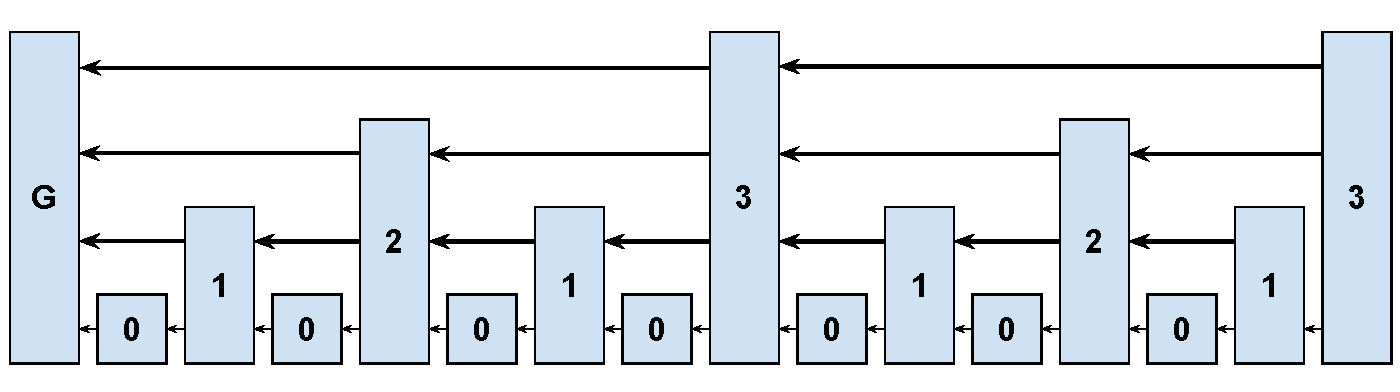
\includegraphics[width=0.7\columnwidth,keepaspectratio]{chapters/superlight/figures/hierarchical-ledger-span.pdf}
    \label{fig.hierarchy}
\end{figure}

The algorithm for this construction is shown in
Algorithm~\ref{alg.interlink-set}~\cite{compactsuperblocks}. The
interlink set of the Genesis block is, by definition, empty. The algorithm
describes how the interlink can be updated once a block is found. The new
interlink is then included in the next block. This construction ensures that
every block contains a direct pointer to its most recent $\mu$-superblock
ancestor, for every $\mu \in \mathbb{N}$.

\import{./}{chapters/superlight/algorithms/alg.interlink-set-update.tex}

The \textsf{updateInterlinkSet} algorithm accepts a block $B'$, which already has an
interlink data structure defined on it. The function evaluates the
interlink data structure which needs to be included as part of the next block.
It copies the existing interlink data structure from level $\textsf{level}(B')$
and adds the reference $H(B')$.

\noindent\textbf{Traversing the blockchain. }
As we have now extended blocks to contain multiple pointers to previous blocks,
if certain blocks are omitted from the middle of a chain we will obtain a
subchain, as long as the \emph{blockchain property} is maintained (i.e., that
each block must contain an interlink pointer to its previous block in the
sequence).

Blockchains are sequences, but it is more convenient to use set notation for
some operations. Let $\chain_1 \cup \chain_2$ be the chain obtained by sorting
the blocks contained in both $\chain_1$ and $\chain_2$ into a sequence (this may
be not always defined, as pointers may be missing). In all cases, the blockchain
property must be maintained. The lowest common ancestor is
$\textsf{LCA}(\chain_1, \chain_2) = (\chain_1 \cap \chain_2)[-1]$. If
$\chain_1[0] = \chain_2[0]$ and $\chain_1[-1] = \chain_2[-1]$, we say the chains
$\chain_1, \chain_2$ \emph{span} the same block range.

It will soon become clear that it is useful to construct a chain containing only
the superblocks of another chain. Given $\chain$ and level $\mu$, the
\emph{upchain} $\chain\upchain^\mu$ is defined as $\{B \in \chain: level(B)
\geq \mu\}$. A chain containing only $\mu$-superblocks is called a
$\mu$\emph{-superchain}. It is also useful, given a $\mu$-superchain $\chain'$
to go back to the \emph{underlying} chain $\chain$ which was used to construct
$\chain'$. Given chains $\chain' \subseteq
\chain$, we will use the \emph{downchain} operator $\chain'\downchain$ to denote
this.
By the above definition, the $\chain\upchain$
operator is absolute: $(\chain\upchain^\mu)\upchain^{\mu + i} =
\chain\upchain^{\mu + i}$. Given a set of consecutive rounds $S = \{r, r + 1,
\cdots, r + j\} \subseteq \mathbb{N}$, we define $\chain^S = \{B \in \chain: B
\text{ was generated during } S\}$. The chain filtering operators~
$\upchain$, $[\cdot]$, and $\{\cdot\}$ have a higher precedence than
$\cup, \cap$.
